\documentclass[]{book}
\usepackage{lmodern}
\usepackage{amssymb,amsmath}
\usepackage{ifxetex,ifluatex}
\usepackage{fixltx2e} % provides \textsubscript
\ifnum 0\ifxetex 1\fi\ifluatex 1\fi=0 % if pdftex
  \usepackage[T1]{fontenc}
  \usepackage[utf8]{inputenc}
\else % if luatex or xelatex
  \ifxetex
    \usepackage{mathspec}
  \else
    \usepackage{fontspec}
  \fi
  \defaultfontfeatures{Ligatures=TeX,Scale=MatchLowercase}
\fi
% use upquote if available, for straight quotes in verbatim environments
\IfFileExists{upquote.sty}{\usepackage{upquote}}{}
% use microtype if available
\IfFileExists{microtype.sty}{%
\usepackage{microtype}
\UseMicrotypeSet[protrusion]{basicmath} % disable protrusion for tt fonts
}{}
\usepackage[margin=1in]{geometry}
\usepackage{hyperref}
\PassOptionsToPackage{usenames,dvipsnames}{color} % color is loaded by hyperref
\hypersetup{unicode=true,
            pdftitle={Coding for Social Scientist},
            pdfauthor={Ujang Fahmi and Canggih Puspo Wibowo},
            colorlinks=true,
            linkcolor=Maroon,
            citecolor=Blue,
            urlcolor=Blue,
            breaklinks=true}
\urlstyle{same}  % don't use monospace font for urls
\usepackage{natbib}
\bibliographystyle{apalike}
\usepackage{color}
\usepackage{fancyvrb}
\newcommand{\VerbBar}{|}
\newcommand{\VERB}{\Verb[commandchars=\\\{\}]}
\DefineVerbatimEnvironment{Highlighting}{Verbatim}{commandchars=\\\{\}}
% Add ',fontsize=\small' for more characters per line
\usepackage{framed}
\definecolor{shadecolor}{RGB}{248,248,248}
\newenvironment{Shaded}{\begin{snugshade}}{\end{snugshade}}
\newcommand{\AlertTok}[1]{\textcolor[rgb]{0.94,0.16,0.16}{#1}}
\newcommand{\AnnotationTok}[1]{\textcolor[rgb]{0.56,0.35,0.01}{\textbf{\textit{#1}}}}
\newcommand{\AttributeTok}[1]{\textcolor[rgb]{0.77,0.63,0.00}{#1}}
\newcommand{\BaseNTok}[1]{\textcolor[rgb]{0.00,0.00,0.81}{#1}}
\newcommand{\BuiltInTok}[1]{#1}
\newcommand{\CharTok}[1]{\textcolor[rgb]{0.31,0.60,0.02}{#1}}
\newcommand{\CommentTok}[1]{\textcolor[rgb]{0.56,0.35,0.01}{\textit{#1}}}
\newcommand{\CommentVarTok}[1]{\textcolor[rgb]{0.56,0.35,0.01}{\textbf{\textit{#1}}}}
\newcommand{\ConstantTok}[1]{\textcolor[rgb]{0.00,0.00,0.00}{#1}}
\newcommand{\ControlFlowTok}[1]{\textcolor[rgb]{0.13,0.29,0.53}{\textbf{#1}}}
\newcommand{\DataTypeTok}[1]{\textcolor[rgb]{0.13,0.29,0.53}{#1}}
\newcommand{\DecValTok}[1]{\textcolor[rgb]{0.00,0.00,0.81}{#1}}
\newcommand{\DocumentationTok}[1]{\textcolor[rgb]{0.56,0.35,0.01}{\textbf{\textit{#1}}}}
\newcommand{\ErrorTok}[1]{\textcolor[rgb]{0.64,0.00,0.00}{\textbf{#1}}}
\newcommand{\ExtensionTok}[1]{#1}
\newcommand{\FloatTok}[1]{\textcolor[rgb]{0.00,0.00,0.81}{#1}}
\newcommand{\FunctionTok}[1]{\textcolor[rgb]{0.00,0.00,0.00}{#1}}
\newcommand{\ImportTok}[1]{#1}
\newcommand{\InformationTok}[1]{\textcolor[rgb]{0.56,0.35,0.01}{\textbf{\textit{#1}}}}
\newcommand{\KeywordTok}[1]{\textcolor[rgb]{0.13,0.29,0.53}{\textbf{#1}}}
\newcommand{\NormalTok}[1]{#1}
\newcommand{\OperatorTok}[1]{\textcolor[rgb]{0.81,0.36,0.00}{\textbf{#1}}}
\newcommand{\OtherTok}[1]{\textcolor[rgb]{0.56,0.35,0.01}{#1}}
\newcommand{\PreprocessorTok}[1]{\textcolor[rgb]{0.56,0.35,0.01}{\textit{#1}}}
\newcommand{\RegionMarkerTok}[1]{#1}
\newcommand{\SpecialCharTok}[1]{\textcolor[rgb]{0.00,0.00,0.00}{#1}}
\newcommand{\SpecialStringTok}[1]{\textcolor[rgb]{0.31,0.60,0.02}{#1}}
\newcommand{\StringTok}[1]{\textcolor[rgb]{0.31,0.60,0.02}{#1}}
\newcommand{\VariableTok}[1]{\textcolor[rgb]{0.00,0.00,0.00}{#1}}
\newcommand{\VerbatimStringTok}[1]{\textcolor[rgb]{0.31,0.60,0.02}{#1}}
\newcommand{\WarningTok}[1]{\textcolor[rgb]{0.56,0.35,0.01}{\textbf{\textit{#1}}}}
\usepackage{longtable,booktabs}
\usepackage{graphicx,grffile}
\makeatletter
\def\maxwidth{\ifdim\Gin@nat@width>\linewidth\linewidth\else\Gin@nat@width\fi}
\def\maxheight{\ifdim\Gin@nat@height>\textheight\textheight\else\Gin@nat@height\fi}
\makeatother
% Scale images if necessary, so that they will not overflow the page
% margins by default, and it is still possible to overwrite the defaults
% using explicit options in \includegraphics[width, height, ...]{}
\setkeys{Gin}{width=\maxwidth,height=\maxheight,keepaspectratio}
\IfFileExists{parskip.sty}{%
\usepackage{parskip}
}{% else
\setlength{\parindent}{0pt}
\setlength{\parskip}{6pt plus 2pt minus 1pt}
}
\setlength{\emergencystretch}{3em}  % prevent overfull lines
\providecommand{\tightlist}{%
  \setlength{\itemsep}{0pt}\setlength{\parskip}{0pt}}
\setcounter{secnumdepth}{5}
% Redefines (sub)paragraphs to behave more like sections
\ifx\paragraph\undefined\else
\let\oldparagraph\paragraph
\renewcommand{\paragraph}[1]{\oldparagraph{#1}\mbox{}}
\fi
\ifx\subparagraph\undefined\else
\let\oldsubparagraph\subparagraph
\renewcommand{\subparagraph}[1]{\oldsubparagraph{#1}\mbox{}}
\fi

%%% Use protect on footnotes to avoid problems with footnotes in titles
\let\rmarkdownfootnote\footnote%
\def\footnote{\protect\rmarkdownfootnote}

%%% Change title format to be more compact
\usepackage{titling}

% Create subtitle command for use in maketitle
\newcommand{\subtitle}[1]{
  \posttitle{
    \begin{center}\large#1\end{center}
    }
}

\setlength{\droptitle}{-2em}

  \title{Coding for Social Scientist}
    \pretitle{\vspace{\droptitle}\centering\huge}
  \posttitle{\par}
  \subtitle{Disampaikan dalam Workshop \emph{Big Data} yang diselenggarakan oleh
CDC, FISIPOL, UGM, 2018}
  \author{Ujang Fahmi and Canggih Puspo Wibowo}
    \preauthor{\centering\large\emph}
  \postauthor{\par}
      \predate{\centering\large\emph}
  \postdate{\par}
    \date{2018-10-31}

\usepackage{booktabs}
\usepackage{amsthm}
\makeatletter
\def\thm@space@setup{%
  \thm@preskip=8pt plus 2pt minus 4pt
  \thm@postskip=\thm@preskip
}
\makeatother

\begin{document}
\maketitle

{
\hypersetup{linkcolor=black}
\setcounter{tocdepth}{1}
\tableofcontents
}
\hypertarget{selamat-datang}{%
\chapter*{Selamat Datang}\label{selamat-datang}}
\addcontentsline{toc}{chapter}{Selamat Datang}

\hypertarget{pengantar}{%
\chapter*{Pengantar}\label{pengantar}}
\addcontentsline{toc}{chapter}{Pengantar}

Saat ini sumber data yang dapat digunakan baik untuk tujuan penelitian
maupun bisnis banyak tersedia di internet. Sayangnya, tidak semua orang
bisa memanfaatkannya. Terdapat beberapa kendala mengapa tidak semua
orang bisa mengekstrak pengetahuan dari sumber data yang cenderung lebih
murah dan sebenarnya mudah untuk di dapatkan tersebut. Salah satu sebab
utamanya kurangnya keterampilan untuk membuat alat untuk mengambilnya.
Dalam konteks ini adalah keterampilan untuk memanfaatkan open source,
salah satunya adalah R.

R merupakan salah satu open source yang saat ini cukup populer dan
banyak digunakan oleh berbagai organisasi dengan skala besar hingga
kecil. Pengguna R tersebar mulai dari perusahaan seperti Google dan
Facebook, pemerintahan, hingga usaha kecil menengah. Berdasarkan
definisi di laman resminya, R merupakan bahasa pemrograman untuk
mengolah data secara statistik. Dalam praktinya R juga banyak digunakan
untuk mengolah data tidak terstruktur, termasuk data dari media sosial.

Sayangnya, \emph{coding} diidentikan hanya dilakukan oleh anak teknik.
Hanya sedikit akademisi sosial yang memiliki kemampuan tersebut.
Padahal, akademisi sosial memiliki salah satu modal utama untuk bisa
membuat data menjadi lebih berarti, yaitu \emph{domain knowledge}.
Sebaliknya, hanya sedikit yang bisa \emph{coding} memiliki \emph{domain
knowledge} untuk bisa memanfaatkan informasi yang diekstrak dari data
dalam jumlah banyak. Dalam konteks ini, kolaborasi lintas disiplin ilmu
dapat menjadi salah satu solusi. Tapi, masing-masing pihak minimal
memiliki pengetahuan dan pemahaman dasar tentang cara kerja
masing-masing. Selain itu, akademisi sosial juga bisa belajar sendiri
dengan memanfaatkan berbagai sumber baik yang gratis maupun berbayar
yang saat ini banyak tersedia di Interent.

Melalui workshop ini, kami bertujuan untuk mengenalkan beberapa dasar
pengelolaan big data dengan menggunakan bahasa pemrograman R. Setelah
mengikuti workhshop, peserta diharapkan memiliki:

\begin{enumerate}
\def\labelenumi{\arabic{enumi}.}
\tightlist
\item
  Pengetahuan tentang bahasa pemrograman;
\item
  Pemahaman alur pengolahan big data; dan
\item
  Kemampuan untuk membuat skrip/menjalankan skrip untuk mendapatkan data
  dari internet
\end{enumerate}

Workshop ini terdiri dari tiga kegiatan. \emph{Pertama}, penjelasan
tentang R dan Rstudio. \emph{Kedua}, memahami proses ekstraksi informasi
dari big data. \emph{Ketiga}, praktik mendapatkan dan mengeksplorasi
data dari twitter.

\hypertarget{pengenalan-dasar}{%
\chapter{Pengenalan dasar}\label{pengenalan-dasar}}

Sebelum melangkah lebih jauh, mungkin kita terlebih dahulu perlu
mengetahui apa itu bahasa pemrograman? apakah ia merupakan bahasa yang
berfungsi sama dengan bahasa yang kita gunakan sehari-hari? Menurut
\href{https://en.wikipedia.org/wiki/Programming_language}{Wikipedia},
bahasa pemrograman adalah:

\begin{quote}
\ldots{} a formal language, which comprises a set of instructions used
to produce various kinds of output. Programming languages are used to
create programs that implement specific algorithms.
\end{quote}

Berdasarkan definisi di atas, maka fungsi bahasa pemrograman kurang
lebih sama dengan bahasa yang kita gunakan sehari-hari dalam membuat
buku petunjuk atau resep masakan. Perbedaannya, bahasa yang kita gunakan
ditujukan agar dapat dipahami oleh manusia, sedangkan bahasa pemrograman
agar dapat dipahami oleh komputer, di mana \texttt{R} merupakan salah
satu di antara bahasa pemrograman yang saat ini ada dan berkembang
dengan pesat.

Sementara \texttt{Rstudio} adalah alat untuk mempermudah penggunaan
\texttt{R}. Di sini \texttt{RStudio} sering disebut sebagai
\emph{integrated development environment} (IDE) untuk R. Sederhananya,
RStudio digunakan sebagai tampilan dari R. Oleh karena itu, untuk
menggunakannya pun kita terlebih dahulu harus menginstall \texttt{R}.
Gambar \texttt{1.1} menunjukkan tampilan antar muka \texttt{Rstudio}
yang perlu diperhatikan.

\begin{figure}
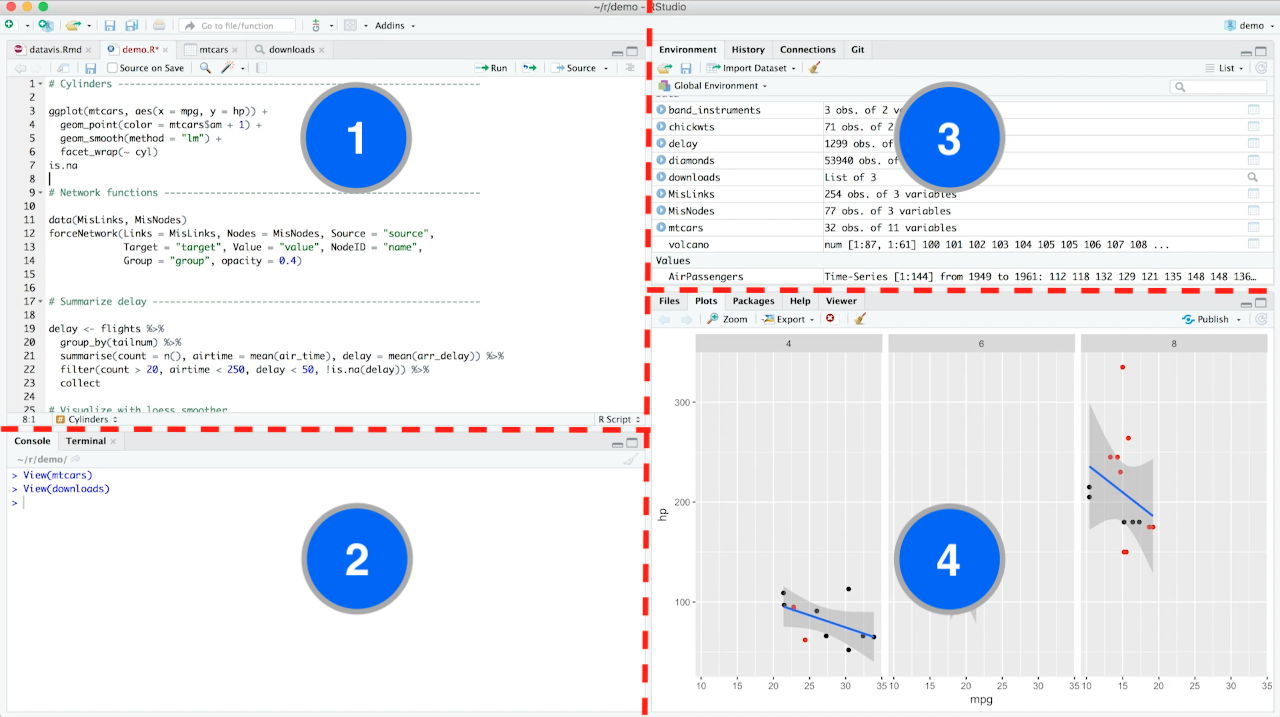
\includegraphics[width=1\linewidth]{images/RStudio} \caption{RStudio Interface terdiri empat bagian utama.}\label{fig:intro1}
\end{figure}

Seperti dapat dilihat pada gambar \texttt{1.1}. Rstudio memiliki empat
bagian yang memiliki fungsi masing-masing. Bagian pertama (1): digunakan
untuk menulis script dan memiliki beberapa tombol. Untuk menjalankan
script bisa klik run pada bagian kanan atas. Bagian kedua (2) :
merupakan bagian \texttt{console} di mana kita bisa melihat script yang
dijalankan. Bagian ketiga (3): merupakan bagian environment, dimana pada
bagian tersebut terdapat beberapa bagian yang bisa pilih. Misalnya,
bagian \texttt{Environment} untuk menampilkan data yang dimasukkan
(diimport), bagian \texttt{Hystory} untuk melihat aktivitas yang sudah
dilakukan dalam satu sesi R, dan bagian \texttt{Connection} untuk
melihat dan mengatur koneksi R dengan database seperti \texttt{SQL} atau
\texttt{SPARK}.

Bagian terakhir (4): berfungsi untuk menampilkan hasil visualiasi
(\texttt{plot}). Selain itu, pada bagian ini kita juga bisa melihat
repository dan file-file yang ada di dalamnya. Lebih penting lagi, di
sini kita juga dapat menemukan bantuan ketika kita lupa instruksi yang
dibutuhkan. Untuk menemukan bantun atau penjelasan kita dapat
menggunakan fungsi \texttt{?} diikuti dengan objek yang ingin dilihat.
Contohnya adalah sebagai berikut.

\begin{Shaded}
\begin{Highlighting}[]
\NormalTok{?read.csv}
\end{Highlighting}
\end{Shaded}

Dengan menuliskan code di atas pada bagian \texttt{console} dan menekan
\texttt{Enter} pada bagian 4 akan menampilkan hasilnya. Di mana pada
tampilan tersebuk kita bisa mendapatkan definisi fungsi sekaligus contoh
penggunaannya. Selain itu, anda juga perlu mencoba untuk menggunakan
fungsi bantuan lainnya, yaitu \texttt{help()} pada console dan lihat apa
yang dihasilkan.

Sebagai rangkuman, pada bagian ini kita sudah mengetahui dan mengenal
beberapa bagian. Pertama untuk menggunakan \texttt{RStudio} kita
terlebih dahulu perlu menginstall \texttt{R}. Untuk mendapatkan bantuan
penjelasan kita bisa menggunakan fungsi \texttt{help()} atau \texttt{?}
diikuti objek yang ingin dilihat. Rstudi terdiri dari beberapa. Untuk
ini saya sarankan untuk mengeksplorasinya lebih jauh, karena pada bagian
selanjutnya kita akan mulai belajar untuk menulis dan menjalankan
script.

\hypertarget{menyiapkan-r}{%
\section{Menyiapkan R}\label{menyiapkan-r}}

Agar dapat menggunakan R secara lokal atau PC/laptop masing-masing, kita
perlu mengunduh installernya terlebih dahulu di laman berikut:

\begin{enumerate}
\def\labelenumi{\arabic{enumi}.}
\tightlist
\item
  Dari Indonesia, R bisa didapat secara gratis di laman:
  \url{https://repo.bppt.go.id/cran/}
\item
  Rstudio dapat didownload melalui laman:
  \url{https://www.rstudio.com/products/rstudio/download/\#download}
\end{enumerate}

Kita bisa menyesuaikan file installer yang sesuai dengan machine
laptop/PC masing, misalnya untuk \texttt{MAC}, \texttt{WINDOWS} atau
\texttt{LINUX}. Setelah dua file tersebut terunduh silahkan install
\texttt{R} terlebih dahulu kemudian \texttt{RStudio}. Setelah keduanya
berhasil di install saat ini mesin pc/latop, jalankan Rstudio.
Selanjutnya coba tuliskan script dibawah ini pada bagian
\texttt{console} lalu tekan \texttt{enter}.

\begin{Shaded}
\begin{Highlighting}[]
\NormalTok{?help}
\NormalTok{?base}
\end{Highlighting}
\end{Shaded}

Script di atas akan mengarahkan anda pada sebuah halaman baru yang
berisi keterangan tentang package dasar \citep{R-base} pada bagian kolom
1 dan keterangan fungsi-fungsi dasar pada kolom 4. Pada bagian kolom 4
ada tulisan \texttt{{[}Package\ base\ version\ 3.5.1\ Index{]}}, klik
bagian \texttt{index} yang berwarna biru dan anda akan diarahkan pada
dokumentasi fungsi-fungsi dasar R. Klik salah satu fungsi untuk membaca
penjelasn dan melihat contoh penggunaannya.

\hypertarget{install-package}{%
\subsection{Install Package}\label{install-package}}

Seperti telah dijelaskan dalam pengantar, pengolahan data dengan R
didukung oleh berbagaik packages atau library yang dokumentasinya dapat
dilihat di laman ini:
\url{https://cran.r-project.org/web/packages/available_packages_by_name.html}.
Untuk dapat menggunakannya anda perlu menginstallnya terlebih dahulu.
Hal ini bisa dilakukan dengan menggunakan salah satu fungsi dasar R,
yaitu \texttt{install.packages()}, di dalam kurung di isi dengan nama
package/library. Misalnya, nama package yang akan diinstall adalah
\texttt{tidyverse} \citep{R-tidyverse}, maka pada bagian
\texttt{console} kita bisa menuliskan script berikut lalu klik enter.

\begin{Shaded}
\begin{Highlighting}[]
\KeywordTok{install.packages}\NormalTok{(}\StringTok{"tidyverse"}\NormalTok{)}
\end{Highlighting}
\end{Shaded}

Agar dapat menginstall package, pc/laptop kita harus terhubung dengan
internet karena R akan mendownload dari laman \texttt{CRAN} di atas.
Selam proses menginstall sebaiknya kita tidak menyimpan script apapun.
Barus setelah selasai menginstall kita bisa melanjutkan aktivitas di
RStudio. Kita dapat mengetahui instalasi sudah selese dengan
memperhatikan bagian console yang akan mengeprint aktivitas yang sedang
berlangsung. Selain itu, pada bagian \texttt{console} sebelah kanan atas
juga ada tanda merah jika masih ada proses yang berlangsung.

Selain dengan menggunakan fungsing \texttt{install.packages()},
packaages atau library juga diinstall dengan menggunakan fitur yang
sematkan di RStudi, yaitu fitur \texttt{Tools}. Fitur \texttt{Tools}
terletak dibagian atas antar muka, dan kita hanya perlu memilih menu
\texttt{install\ packages} yang ada di dalamnya dan akan muncul kota
dialog baru seperti di terlihat pada gambar berikut.

\begin{figure}
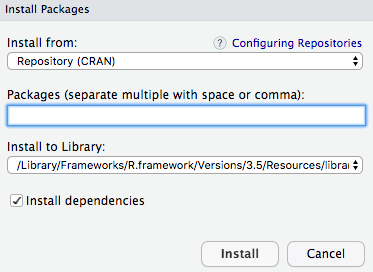
\includegraphics[width=0.4\linewidth]{images/installpackage} \caption{RStudio Interface terdiri empat bagian utama.}\label{fig:intro5}
\end{figure}

Dialog box seperti pada gambar 1.2 menunjukkan ada tiga isian yang perlu
diperhatikan. Pertama, bagian sumber. Secara \emph{default} sumber
package yang akan diinstall diambil dari CRAN. Kedua, kolom nama package
yang harus diisi secara manual (ketik). Ketiga, kolom yang menunjukkan
\emph{repository} atau folder tempat package akan diinstall. Keemapat,
dependency yang ketika dicentang berarti kita akan menginstal package
atau library lain yang dibutuhkan oleh package yang akan diinstall.
Untuk sementara, dua kolom yang disebut terakhir disarankan untuk
biarkan pengaturan semula atau \emph{default}.

\hypertarget{latihan-1}{%
\subsection{Latihan 1}\label{latihan-1}}

\begin{quote}
Untuk mengelola teks, terdapat salah satu library dengan nama
\texttt{tidytext}. Installah library tersebut dengan salah satu metode
install package yang sudah dijelaskan.
\end{quote}

\hypertarget{simbol-simbol-utama}{%
\subsection{Simbol-simbol utama}\label{simbol-simbol-utama}}

Secara lengkapnya, simbol dan fungsi-fungsi dasar dapat dipelajari
\href{https://www.rstudio.com/wp-content/uploads/2016/05/base-r.pdf}{di
sini}. Namun pada umumnya, dalam \texttt{R} ada dua simbol utama yang
sering digunakan yaitu \texttt{"xyz"} (tanda petik) dan \texttt{\#}
(tanda pagar).

\begin{enumerate}
\def\labelenumi{\arabic{enumi}.}
\tightlist
\item
  Tanda petik (\texttt{"xyz"}) digunakan untuk menunjukkan bahwa apapun
  yang ada diantara dua tanda petik tersebut dianggap sebagai character
  (\texttt{chr}). Sebagai contoh, jalankan script di bawah ini.
\end{enumerate}

\begin{Shaded}
\begin{Highlighting}[]
\CommentTok{# vector}
\NormalTok{huruf_a <-}\StringTok{ "1"}
\CommentTok{# cek apakah karakter atau bukan}
\KeywordTok{is.character}\NormalTok{(huruf_a)}
\end{Highlighting}
\end{Shaded}

\begin{verbatim}
## [1] TRUE
\end{verbatim}

\begin{Shaded}
\begin{Highlighting}[]
\CommentTok{# vector}
\NormalTok{huruf_b <-}\StringTok{ }\DecValTok{1}
\CommentTok{# cek apakah karakter atau bukan}
\KeywordTok{is.character}\NormalTok{(huruf_b)}
\end{Highlighting}
\end{Shaded}

\begin{verbatim}
## [1] FALSE
\end{verbatim}

\begin{enumerate}
\def\labelenumi{\arabic{enumi}.}
\setcounter{enumi}{1}
\item
  Tanda pagar (\texttt{\#}) digunakan untuk memberikan komentar yang
  berfungsi untuk memberikan keterangan terhadap script yang kita buat.
  Sebagai contoh, pada script di atas term vector yang didahului oleh
  tanda pagar saya gunakan untuk mengingat bahwa kode yang ada
  dibahwanya merupakan sebuah vector. Sementara komentar berikutnya saya
  gunakan untuk memberikan keterangan bahwa kode yang ada dibawahnya
  digunkan untuk mengecek apakah benar \texttt{huruf\_a} dan
  \texttt{huruf\_b} merupakan karakter.
\item
  Tanda \texttt{\textless{}-} atau \texttt{=} dibaca sama dengan.
\end{enumerate}

\hypertarget{membuat-skrip-r}{%
\section{Membuat skrip R}\label{membuat-skrip-r}}

Dengan menggunakan \texttt{RStudio} kita bisa membuat beberja jenis
script untuk menuliskan bahasa R. Untuk sementara saya hanya akan
mengenalkan dua jenis dulu, yaitu \texttt{.R}. Caranya adalah dengan
klik menu \texttt{File} -\textgreater{} \texttt{New\ file}
-\textgreater{} \texttt{R\ Script} atau \texttt{Command+Shift+N} jika
menggunakan Macbook. Sama seperti saat kita menulis atau membuat file
pada umumnya, pada saat menulis script R untuk mengorganisasinya dengan
mudah kita perlu meletakannya dalam sebuah folder atau \emph{repository}
khusus. Di dalam RStudio, kita bisa membuatnya dengan memilih
\texttt{New\ Project...} pada menu file, lalu pilih
\texttt{New\ Directory} dan pilih \texttt{New\ Project}. Setelah itu,
kita bisa menentukan hardisk yang akan digunakan untuk menyimpan file
\emph{project} yang sedang dikerjakan, menamai folder, dan lain
sebagainya. Dengan cara seperti itu, pekerjaan kita bisa menjadi lebih
terorganisasi.

\begin{Shaded}
\begin{Highlighting}[]
\CommentTok{# Untuk memastikan di mana kita menyimpan file atau project}
\KeywordTok{getwd}\NormalTok{()}
\end{Highlighting}
\end{Shaded}

\hypertarget{latihan-2}{%
\subsection{Latihan 2}\label{latihan-2}}

\begin{quote}
Buatlah sebuah proyek baru dengan nama yang anda pilih sendiri. Setelah
itu, buat sebuah R script dan simpan dalam project tersebut.
\end{quote}

\hypertarget{menulis-skrip}{%
\subsection{Menulis skrip}\label{menulis-skrip}}

Untuk memulai menulis skrip, terdapat dua hal pertama yang ingin saya
anggap sebagai dasar, yaitu cara membuat variabel dan mengenal jenis
data. Terkait dengan jenis data, terdapat beberapa data yang bisa
digunakan seperti vector, data frame, lists, dan matrix. Di sini kita
akan lebih fokus ke vector dan data frame saja. Namun jika tertarik
untuk mempelajarinya lebih lanjut bisa memulainya
\href{https://www.r-bloggers.com/basic-data-types-in-r/}{di sini}.

\begin{itemize}
\tightlist
\item
  \textbf{Nama file}
\end{itemize}

Dalam membuat variabel atau nama file di R tidak boleh ada spasi. Selain
itu R juga case sensitve. Sebagi contoh kita ingin menamai file dengan
nama \textbf{\texttt{Data\ Kita}} akan menyebabkan error karena ada
spasi. Sebaiknya jika ingin menggunakan dua term atau elemen
menyambungnya dengan \texttt{\_} seperti: \textbf{\texttt{Data\_Kita}}.
Berikut adalah contohnya:

\begin{Shaded}
\begin{Highlighting}[]
\NormalTok{Data_Kita <-}\StringTok{ }\NormalTok{mtcars}
\end{Highlighting}
\end{Shaded}

Keterangan: skrip di atas mengambil data dengan nama mtcars, yang
merupakan data bawaan dari R, sebagai data dengan nama Data\_Kita.

\begin{itemize}
\tightlist
\item
  \textbf{Data frame}
\end{itemize}

Sebuah data frame pada prinsipnya adalah sebuah tabel di mana setiap
kolom memiliki satu jenis variable dan setiap baris (\emph{row})
mengandung satu nilai untuk masing-masing variabel/kolom. Berikut ini
adalah karakteristik dari suatu frame data yang contohnya dapat dilihat
pada tabel \ref{tab:contohtable}.

\begin{enumerate}
\def\labelenumi{\arabic{enumi}.}
\tightlist
\item
  Memiliki nama kolom
\item
  Nama baris harus unik
\item
  Data yang disimpan dalam data frame dapat berupa angka, faktor atau
  karakter
\item
  Setiap kolom memiliki item data yang sama
\end{enumerate}

\begin{table}

\caption{\label{tab:contohtable}Contoh Isi sebuah data frame}
\centering
\begin{tabular}[t]{l|l|l}
\hline
name & genus & vore\\
\hline
Cheetah & Acinonyx & carni\\
\hline
Owl monkey & Aotus & omni\\
\hline
Mountain beaver & Aplodontia & herbi\\
\hline
Greater short-tailed shrew & Blarina & omni\\
\hline
Cow & Bos & herbi\\
\hline
\end{tabular}
\end{table}

Untuk melihat rangkuman dan jenis sebuah data kita bisa menggunakan
\texttt{summary()} dan \texttt{class()}. Untuk melihat struktur sebuah
data bisa menggunakan fungsi \texttt{str()}.

\begin{itemize}
\tightlist
\item
  \textbf{Menjalankan skrip}
\end{itemize}

Untuk menjalankan skrip R yang sudah kita tulis, kita bisa menggunakan
\emph{shortcut}. Jika menggunakan mac, kita blok bari skrip yang akan
dijalankan dan tekan command+shift+enter. Selain itu kita bisa
menggunakan tombol run dibagian kanan atas.

\textbf{Lathian:} Coba jalankan skrip di bawah ini dan lihat hasil dari
tiga fungsi di atas, yaitu \texttt{summary()}, \texttt{class()}, dan
\texttt{str()} pada data tentang pola tidur yang sudah ada dalam
Rstudio.

\begin{Shaded}
\begin{Highlighting}[]
\NormalTok{data <-}\StringTok{ }\NormalTok{msleep }\CommentTok{# data}

\KeywordTok{str}\NormalTok{(data)}
\KeywordTok{class}\NormalTok{(data)}
\KeywordTok{summary}\NormalTok{(data)}
\end{Highlighting}
\end{Shaded}

\hypertarget{tidyverse}{%
\subsection{Tidyverse}\label{tidyverse}}

Tidyverse merupakan kumpulan packages yang terdiri dari beberapa package
lain, seperty \texttt{readr}, \texttt{dplyr}, \texttt{ggplot} dan
beberapa package lainnya. Ketika menggunakan R untuk mengolah data atau
mengeksplorasi data kita akan banyak menggunakan package-package ini.
Secara keseluruhan, dalam modul ini saya akan mengenalakan beberapa
fungsi dari tiga package yang disebutkan di atas dalam beberapa bagian
yang berebeda sesuai dengan fungsinya.

Pertama, readr akan lebih banyak digunakan untuk mengimpor data. Kedua,
dplyr akan lebih banyak digunakan dalam melakukan pre-processing.
Sementara ggplot akan sangat membantu dalam melakukan eksplorasi dengan
visualisasi. Di sini saya akan lebih fokus untuk menjelaskan
\texttt{dplyr} terlebih dahulu.

\texttt{dplyr} memiliki fungsi pipe yang tandangnya adalah
\texttt{\%\textgreater{}\%} yang berfungsi untuk mengaplikasikan baris
berikutnya pada baris sebelumnya. Sebagai contoh dapat dilihat pada
skrip di bawah ini.

\begin{Shaded}
\begin{Highlighting}[]
\KeywordTok{library}\NormalTok{(dplyr)}

\NormalTok{data <-}\StringTok{ }\NormalTok{msleep }\OperatorTok
\StringTok{  }\KeywordTok{select}\NormalTok{(}\DecValTok{1}\OperatorTok{:}\DecValTok{3}\NormalTok{)}
\end{Highlighting}
\end{Shaded}

Skrip di atas kita mengambil \texttt{msleep} yang kita sebuat sebagai
\texttt{data}, lalu kita hanya memilih kolom nomor 1 sampai tiga saja
dari data. Fungsi \texttt{select()} di sini berfungsi untuk memilih.
Berikutnya adalah beberapa fungsi lain yang mungkin akan sering
digunakan dalam proses belajar kita.

\texttt{select()}: pick columns by name

\texttt{filter()}: keep rows matching criteria

\texttt{arrange()}: reorder rows

\texttt{mutate()}: add new variables

\texttt{summarise()}: reduce variables to values

Untuk belejar lebih lanjut untuk fungsi yang dimiliki oleh masing-masing
package kita bisa menggunakan skrip di bawah ini. Misalnya kita ingin
belajar tentang dplyr. Untuk package lain kita hanya perlu mengganti
\texttt{dplyr} dan \texttt{readr} dengan nama package lainnya.

\begin{Shaded}
\begin{Highlighting}[]
\KeywordTok{browseVignettes}\NormalTok{(}\DataTypeTok{package =} \StringTok{"dplyr"}\NormalTok{)}
\KeywordTok{browseVignettes}\NormalTok{(}\DataTypeTok{package =} \StringTok{"readr"}\NormalTok{)}
\end{Highlighting}
\end{Shaded}

\hypertarget{rangkuman}{%
\section{Rangkuman}\label{rangkuman}}

Beberapa hal dasar yang telah sampaikan pada bagian ini adalah:

\begin{enumerate}
\def\labelenumi{\arabic{enumi}.}
\tightlist
\item
  R bisa digunakan dengan RStudio yang bisa di dapat secara gratis
\item
  Dalam mengolah data di R kita terbantu dengan package dan library yang
  ada yang dapat dinstall dengan menggunakan fungsi
  \texttt{install.package()}
\item
  Agar skrip lebih mudah dibaca dan dipahami kita bisa menambahkan
  komentar dengan didahului tanda pagar \texttt{\#}
\item
  Untuk memulai menulis skrip kita sebaiknya terlebih dahulu membuat
  project dalam folder yang spesifik yang semuanya bisa diakses melalui
  menu \texttt{File}
\item
  Menggunakan library tidyverse dalam pengolahan data
\item
  Mengetahui beberapa fungsi dasar dan dari tidyverse yang cenderung
  akan lebih banyak digunakan seperti \texttt{class()}, \texttt{str()},
  \texttt{summary()} dan beberapa fungsi lainnya yang bisa dipelajari
  lebih lanjut melalui dokumentasi yang disediakan pembuat package dan
  dapat diakses baik dengan menggunakan fungsi \texttt{help()} maupun
  \texttt{browseVignettes(package\ =\ "dplyr")}.
\end{enumerate}

\hypertarget{proses-ekstraksi-informasi}{%
\chapter{Proses Ekstraksi Informasi}\label{proses-ekstraksi-informasi}}

Pada bagian ini kita akan mempelajari bagaimana cara untuk mengekstrak
informasi dari teks sosial media, terutama Twitter. Ada empat langkah
utama dalam tahap ini, yaitu: impor/ekspor data, preprocessing,
eksplorasi, dan visualisasi. Kita akan membahas secara singkat
masing-masing langkah.

\hypertarget{impor-dan-ekspor-data}{%
\section{Impor dan Ekspor Data}\label{impor-dan-ekspor-data}}

Pada pengolahan data menggunakan R, direkomendasikan menggunakan tipe
data file CSV (\texttt{Comma\ Separated\ Value}). Secara sederhana, file
CSV merupakan file tabel yang serupa dengan XLS namun dengan variasi
delimiter atau pemisah nilai. File CSV dapat diolah sebagaimana XLS
dalam aplikasi Microsoft Excel.

\hypertarget{membaca-data-import}{%
\subsection{Membaca data (Import)}\label{membaca-data-import}}

Untuk membaca file CSV dalam lingkungan R, ada banyak cara yang bisa
dilakukan. Cara pertama yaitu dengan menggunakan fungsi yang sudah
tersedia pada R, yaitu \texttt{read.csv()} dengan contoh perintah
sebagai berikut

\begin{Shaded}
\begin{Highlighting}[]
\NormalTok{df <-}\StringTok{ }\KeywordTok{read.csv}\NormalTok{(nama_file_csv)}
\end{Highlighting}
\end{Shaded}

Cara tersebut dapat digunakan untuk membaca CSV berukuran kecil.
Sedangkan bila kita ingin membaca file CSV berukuran relatif besar,
direkomendasikan menggunakan library \texttt{readr} seperti yang sudah
disinggung pada bab sebelumnya. Penggunaan library ini memungkinkan file
dibaca jauh lebih cepat dibandingkan metode sebelumnya. Perintah yang
digunakan adalah

\begin{Shaded}
\begin{Highlighting}[]
\NormalTok{df <-}\StringTok{ }\NormalTok{readr}\OperatorTok{::}\KeywordTok{read_csv}\NormalTok{(nama_file_csv)}
\end{Highlighting}
\end{Shaded}

Hasil pembacaan yang disimpan dalam \texttt{df} merupakan sebuah data
tabel.

\hypertarget{menyimpan-data-ekspor}{%
\subsection{Menyimpan data (Ekspor)}\label{menyimpan-data-ekspor}}

Kita dapat menggunakan fungsi dari \texttt{readr} yaitu
\texttt{write\_csv()} untuk menyimpan data tabel ke dalam file CSV.
Perintah yang digunakan adalah sebagai berikut:

\begin{Shaded}
\begin{Highlighting}[]
\NormalTok{readr}\OperatorTok{::}\KeywordTok{write_csv}\NormalTok{(nama_file_csv)}
\end{Highlighting}
\end{Shaded}

\hypertarget{menampilkan-data}{%
\subsection{Menampilkan data}\label{menampilkan-data}}

Untuk menampilkan data, disediakan perintah \texttt{print()}. Contoh
penggunaannya sebagai berikut:

\begin{Shaded}
\begin{Highlighting}[]
\KeywordTok{print}\NormalTok{(df)}
\end{Highlighting}
\end{Shaded}

Perintah di atas akan menampilkan isi dari \texttt{df}. Namun jika
jumlah barisnya banyak, maka data hanya akan ditampilkan beberapa saja.
Untuk menampilkan kolom tertentu dalam suatu data tabel, kita perlu
menambahkan \texttt{\$\textless{}namakolom\textgreater{}} seperti contoh
berikut:

\begin{Shaded}
\begin{Highlighting}[]
\KeywordTok{print}\NormalTok{(df}\OperatorTok{$}\NormalTok{text)}
\end{Highlighting}
\end{Shaded}

Perintah tersebut akan menampilkan kolom \texttt{text} pada data tabel
\texttt{df}.

\hypertarget{pre-processing}{%
\section{Pre-processing}\label{pre-processing}}

Preprocessing merupakan sebuah langkah yang perlu dilakukan sebelum data
siap untuk diproses atau dianalisis. Ada banyak jenis langkah
preprocessing yang dapat dilakukan, namun langkah ini harus disesuaikan
dengan data yang kita miliki. Pada kesempatan ini, kita akan melakukan
preprocessing untuk teks yang berasal dari media sosial.

\hypertarget{menghapus-karakter-non-ascii}{%
\subsection{Menghapus karakter
non-ASCII}\label{menghapus-karakter-non-ascii}}

Karakter teks yang digunakan di Indonesia menggunakan standar
\href{https://en.wikipedia.org/wiki/ASCII}{ASCII}, namun pada banyak
negara terdapat karakter-karakter yang tidak terdapat dalam standar
ASCII. Pada kasus tersebut, digunakan standar yang lain, yaitu
\href{https://en.wikipedia.org/wiki/Unicode}{Unicode} yang memiliki
variasi karakter lebih banyak. ASCII pada dasarnya adalah bagian dari
Unicode. Pada teks sosial media, seringkali karakter non-ASCII tertulis
dan itu cukup membuat sulit dalam pengolahan teks, karena kita
menggunakan ASCII. Oleh karena itu, pada langkah pertama preprocessing,
kita harus menghapus karakter non-ASCII tersebut.

Ciri karakter non-ASCII yang terlihat adalah adanya format seperti
\texttt{\textless{}U+...\textgreater{}} pada teks yang kita miliki.
Untuk menghapusnya, kita akan menggunakan perintah
\texttt{global\ substitution} sebagai berikut:

\begin{Shaded}
\begin{Highlighting}[]
\NormalTok{text <-}\StringTok{ }\KeywordTok{gsub}\NormalTok{(}\StringTok{"[<].*[>]"}\NormalTok{, }\StringTok{""}\NormalTok{, text)}
\end{Highlighting}
\end{Shaded}

Perintah di atas bermakna mengganti semua teks dengan format
\texttt{\textless{}..\textgreater{}} dalam variabel \texttt{text} dengan
kosong, atau dengan kata lain, menghapusnya kemudian menyimpannya
kembali ke dalam variabel \texttt{text}. Ini salah satu strategi dalam
menghilangkan karakter non-ASCII

\hypertarget{menghapus-alamat-url}{%
\subsection{Menghapus alamat URL}\label{menghapus-alamat-url}}

Sering kita temui pada teks sosial media, alamat URL sebuah website atau
sejenisnya. Tentu kita tidak memerlukan alamat URL ini pada analisis
selanjutnya. Untuk menghapusnya, bisa digunakan perintah:

\begin{Shaded}
\begin{Highlighting}[]
\NormalTok{text <-}\StringTok{ }\KeywordTok{gsub}\NormalTok{(}\StringTok{'http}\CharTok{\textbackslash{}\textbackslash{}}\StringTok{S+}\CharTok{\textbackslash{}\textbackslash{}}\StringTok{s*'}\NormalTok{,}\StringTok{""}\NormalTok{, text)}
\end{Highlighting}
\end{Shaded}

Dengan menggunakan perintah tersebut, semua teks dengan format
\texttt{http...} (format alamat URL) akan dihapus. \#\#\# Menghapus
tanda baca Tanda baca menjadi hal selanjutnya yang akan kita hapus untuk
mendapatkan teks yang siap untuk dianalisis. Metode yang bisa digunakan
adalah dengan memanfaatkan perintah \texttt{gsub} sama seperti
sebelumnya dengan pola yang berbeda.

\begin{Shaded}
\begin{Highlighting}[]
\NormalTok{text <-}\StringTok{ }\KeywordTok{gsub}\NormalTok{(}\StringTok{"[^[:alnum:][:space:]#@]"}\NormalTok{, }\StringTok{""}\NormalTok{, text)}
\end{Highlighting}
\end{Shaded}

Penjelasan mengenai perintah tersebut * Tanda \texttt{{[}\^{}\ {]}}
bermakna ambil selain pola yang ada di dalam kurung siku * Teks
\texttt{{[}:alnum:{]}} bermakna semua huruf dan angka (alfanumerik) *
Teks \texttt{{[}:space:{]}} bermakna spasi * Karakter \texttt{\#@}
bermakna literal Sehingga perintah itu secara umum bermakna menghapus
semua karakter selain huruf, angka, spasi, \texttt{\#} dan \texttt{@}.
Dua yang terakhir sengaja tidak kita hapus karena akan digunakan untuk
analisis akun dan tagar pada tahap selanjutnya.

\hypertarget{menghapus-tanda-ganti-baris}{%
\subsection{Menghapus tanda ganti
baris}\label{menghapus-tanda-ganti-baris}}

Pada teks sosial media maupun teks pada umumnya, kita akan sering
menjumpai karakter \texttt{\textbackslash{}n} yang merupakan karakter
pindah baris (ada ketika kita menekan \texttt{enter} pada keyboard).
Karakter ini normalnya tidak akan terlihat, namun ketika kita ambil teks
dalam format ASCII, karakter ini akan diterjemahkan menjadi
\texttt{\textbackslash{}n}. Untuk menghapusnya, kita dapat menggunakan
perintah berikut:

\begin{Shaded}
\begin{Highlighting}[]
\NormalTok{text <-}\StringTok{ }\KeywordTok{gsub}\NormalTok{(}\StringTok{"}\CharTok{\textbackslash{}n}\StringTok{"}\NormalTok{,}\StringTok{" "}\NormalTok{,text)}
\end{Highlighting}
\end{Shaded}

Jika diperlukan kita bisa menggunakan cara yang sama untuk menghapus
karakter sejenis lain, misalnya \texttt{\textbackslash{}t} yang berarti
\texttt{tab}. Namun karakter tersebut sangat jarang ada di sosial media
twitter.

\hypertarget{mengubah-ke-huruf-kecil}{%
\subsection{Mengubah ke huruf kecil}\label{mengubah-ke-huruf-kecil}}

Menyeragamkan huruf kapital menjadi hal yang sangat penting dalam
pengolahan teks. Hal ini dikarenakan komputer akan menganggap
\texttt{teks} berbeda dari \texttt{Teks}. Oleh sebab itu, dengan
perintah bawaan R, \texttt{tolower()}, kita akan membuat semua karakter
ke dalam huruf kecil.

\begin{Shaded}
\begin{Highlighting}[]
\NormalTok{text <-}\StringTok{ }\KeywordTok{tolower}\NormalTok{(text)}
\end{Highlighting}
\end{Shaded}

\hypertarget{explorasi1}{%
\section{Eksplorasi}\label{explorasi1}}

Pada eksplorasi ini, kita akan mencoba mencari tahu tentang akun paling
banyak disebut, tagar paling sering digunakan, serta kata yang paling
sering ditulis. Namun sebelumnya satu langkah yang harus dilakukan
adalah proses tokenisasi.

\hypertarget{tokenisasi}{%
\subsection{Tokenisasi}\label{tokenisasi}}

Tokenisasi pada dasarnya adalah proses membagi teks yang berupa kalimat
atau paragraf menjadi bagian-bagian tertentu. Dalam konteks ini, kita
akan membagi kumpulan kalimat ke dalam kumpulan kata-kata. Untuk
melakukan tokenisasi, kita bisa menggunakan metode dari library
\texttt{tidytext} yaitu \texttt{unnest\_tokens()}. Contoh perintahnya
adalah sebagai berikut:

\begin{Shaded}
\begin{Highlighting}[]
\NormalTok{df_new <-}\StringTok{ }\NormalTok{tidytext}\OperatorTok{::}\KeywordTok{unnest_tokens}\NormalTok{(df,word,text,}\DataTypeTok{token=}\StringTok{'regex'}\NormalTok{,}\DataTypeTok{pattern=}\StringTok{"[:space:]"}\NormalTok{)}
\end{Highlighting}
\end{Shaded}

Penjelasan dari kode tersebut adalah sebagai berikut:

\begin{itemize}
\tightlist
\item
  \texttt{df\_new} merupakan data frame tempat menyimpan hasil
  tokenisasi
\item
  \texttt{tidytext::unnest\_tokens} perintah untuk memanfaatkan fungsi
  \texttt{unnest\_tokens} yang berasal dari library \texttt{tidytext}
\item
  \texttt{df} adalah data frame awal yang belum diproses
\item
  \texttt{word} adalah nama kolom yang kita buat untuk menampung hasil
  dari tokenisasi
\item
  \texttt{text} adalah nama kolom dari data frame \texttt{df} dimana
  berisi teks yang akan ditokenisasi
\item
  \texttt{token=\textquotesingle{}regex\textquotesingle{}} berarti kita
  menggunakan metode tokenisasi dengan memanfaatkan pola
  \href{https://en.wikipedia.org/wiki/Regular_expression}{regex}. Regex
  merupakan sebuah pola karakter yang lazim digunakan untuk pencarian
  teks tertentu.
\item
  \texttt{pattern="{[}:space:{]}"} berarti bahwa pola regex yang akan
  kita gunakan adalah spasi. Perintah ini juga bermakna bahwa teks akan
  kita pisah-pisah berdasarkan spasi, sehingga akan menghasilkan
  kata-kata.
\end{itemize}

Hasil dari perintah di atas adalah sebuah data frame \texttt{df\_new}
dengan satu kolom bernama \texttt{word} yang berisi satu kata per baris.
Contohnya dapat dilihat pada Tabel \ref{tab:table1}.

\begin{table}

\caption{\label{tab:table1}Hasil tokenisasi}
\centering
\begin{tabular}[t]{l}
\hline
word\\
\hline
saya\\
\hline
mereka\\
\hline
makan\\
\hline
\end{tabular}
\end{table}

\hypertarget{akun-paling-banyak-disebut}{%
\subsection{Akun paling banyak
disebut}\label{akun-paling-banyak-disebut}}

Untuk mencari siapa akun-akun yang paling banyak disebut dalam menulis
twit, pada dasarnya kita cukup melakukan filter dari data frame hasil
tokenisasi sebelumnya, kemudian menghitung frekuensi munculnya tiap
akun. Pada langkah ini, kita akan menggunakan bantuan fungsi
\texttt{filter()} dari library \texttt{dplyr} dan fungsi
\texttt{str\_detect()} dari library \texttt{stringr}. Contoh
penggunaannya dapat dilihat pada perintah berikut:

\begin{Shaded}
\begin{Highlighting}[]
\NormalTok{df_akun <-}\StringTok{ }\NormalTok{dplyr}\OperatorTok{::}\KeywordTok{filter}\NormalTok{(df_new,stringr}\OperatorTok{::}\KeywordTok{str_detect}\NormalTok{(word, }\StringTok{"@"}\NormalTok{))}
\end{Highlighting}
\end{Shaded}

\begin{itemize}
\tightlist
\item
  \texttt{dplyr::filter()} merupakan fungsi yang digunakan untuk
  melakukan filtering pada data frame sesuai dengan kondisi tertentu
\item
  \texttt{stringr::str\_detect()} digunakan untuk mencari baris tertentu
  pada suatu kolom yang memiliki pola tertentu
\end{itemize}

Perintah di atas bermakna kita hanya akan mengambil baris-baris pada
data frame \texttt{df\_new} kolom \texttt{word} yang mengandung karakter
\texttt{@}, dengan kata lain berupa akun, kemudian hasilnya disimpan
pada \texttt{df\_akun}.

Setelah semua akun terambil, kita dapat menghitung frekuensi
masing-masing dengan mengubah data frame \texttt{df\_akun} ke dalam
format tabel. Secara otomatis R akan menghitung frekuensi dari
masing-masing baris yang sama. Kemudian kita ubah \texttt{df\_akun}
kembali ke data frame untuk bisa ditampilkan dan diolah lebih lanjut.

\begin{Shaded}
\begin{Highlighting}[]
\NormalTok{df_akun <-}\StringTok{ }\KeywordTok{table}\NormalTok{(df_akun)}
\NormalTok{df_akun <-}\StringTok{ }\KeywordTok{as.data.frame}\NormalTok{(df_akun)}
\end{Highlighting}
\end{Shaded}

Selanjutnya untuk mengurutkan data berdasar frekuensi, kita dapat
menggunakan fungsi \texttt{arrange()} dari library \texttt{dplyr}
sebagai berikut.

\begin{Shaded}
\begin{Highlighting}[]
\NormalTok{df_akun <-}\StringTok{ }\NormalTok{dplyr}\OperatorTok{::}\KeywordTok{arrange}\NormalTok{(df_akun,}\KeywordTok{desc}\NormalTok{(Freq))}
\end{Highlighting}
\end{Shaded}

Kode di atas akan menghasilkan data frame \texttt{df\_akun} yang berisi
daftar akun dan frekuensinya yang telah diurutkan secara descending.

\hypertarget{tagar-paling-sering-digunakan}{%
\subsection{Tagar paling sering
digunakan}\label{tagar-paling-sering-digunakan}}

Untuk mencari frekuensi tagar yang digunakan, kita dapat menggunakan
cara yang mirip dengan langkah mencari akun di atas. Hanya saja untuk
filter yang digunakan, karakter \texttt{@} diganti dengan \texttt{\#}
seperti berikut.

\begin{Shaded}
\begin{Highlighting}[]
\NormalTok{df_tagar <-}\StringTok{ }\NormalTok{dplyr}\OperatorTok{::}\KeywordTok{filter}\NormalTok{(df_new,stringr}\OperatorTok{::}\KeywordTok{str_detect}\NormalTok{(word, }\StringTok{"#"}\NormalTok{))}
\end{Highlighting}
\end{Shaded}

Langkah selanjutnya sama dengan sebelumnya.

\hypertarget{kata-paling-sering-ditulis}{%
\subsection{Kata paling sering
ditulis}\label{kata-paling-sering-ditulis}}

Untuk mencari frekuensi kata selain nama akun dan tagar, kita butuh
mengubah pola pencarian yang digunakan. Contoh yang bisa digunakan
adalah sebagai berikut.

\begin{Shaded}
\begin{Highlighting}[]
\NormalTok{df_kata <-}\StringTok{ }\NormalTok{dplyr}\OperatorTok{::}\KeywordTok{filter}\NormalTok{(df_new,stringr}\OperatorTok{::}\KeywordTok{str_detect}\NormalTok{(word, }\StringTok{"^((?!@|#).)*$"}\NormalTok{))}
\end{Highlighting}
\end{Shaded}

Perintah di atas akan mencari kata selain yang berawalan \texttt{@} dan
\texttt{\#} dalam data frame \texttt{df\_new} kemudian menyimpannya ke
dalam data frame \texttt{df\_kata}.

\hypertarget{visualisasi}{%
\section{Visualisasi}\label{visualisasi}}

Untuk visualisasi dari data yang sudah didapat, kita dapat menggunakan
bar chart. Implementasi bar chart dalam R didapat dengan memanfaatkan
library \texttt{ggplot} dengan contoh kode sebagai berikut:

\begin{Shaded}
\begin{Highlighting}[]
\KeywordTok{ggplot}\NormalTok{(}\KeywordTok{head}\NormalTok{(df_akun,}\DataTypeTok{n=}\DecValTok{10}\NormalTok{),}\KeywordTok{aes}\NormalTok{(}\DataTypeTok{x=}\KeywordTok{reorder}\NormalTok{(col_akun,Freq),}\DataTypeTok{y=}\NormalTok{Freq)) }\OperatorTok{+}\StringTok{ }
\StringTok{  }\KeywordTok{geom_col}\NormalTok{() }\OperatorTok{+}\StringTok{ }
\StringTok{  }\KeywordTok{coord_flip}\NormalTok{() }\OperatorTok{+}
\StringTok{  }\KeywordTok{labs}\NormalTok{(}\DataTypeTok{title=}\StringTok{'10 akun paling banyak disebut'}\NormalTok{,}\DataTypeTok{x=}\StringTok{'nama akun'}\NormalTok{,}\DataTypeTok{y=}\StringTok{'jumlah'}\NormalTok{)}
\end{Highlighting}
\end{Shaded}

\begin{itemize}
\tightlist
\item
  \texttt{head(df\_akun,n=10)} maksudnya ialah mengambil 10 baris
  pertama dari data frame \texttt{df\_akun}
\item
  \texttt{aes()} merupakan perintah untuk mendeskripsikan variabel mana
  yang akan ditampilkan dalam sumbu grafik. Perintah
  \texttt{reorder(col\_akun,Freq)} bermakna data pada kolom
  \texttt{col\_akun} akan diurutkan berdasarkan kolom \texttt{Freq}
\item
  \texttt{geom\_col()} merupakan perintah yang bermakna grafik yang kita
  buat merupakan bar chart
\item
  \texttt{coord\_flip()} merupakan perintah untuk menukar sumbu pada
  grafik. Pada kasus ini, kita menggunakan perintah ini untuk membuat
  horizontal bar chart
\item
  \texttt{labs()} digunakan untuk memberi label
\end{itemize}

\hypertarget{latihan}{%
\chapter{Latihan}\label{latihan}}

Dalam latihan kali ini terdapat dua hal utama yang akan kita coba.
Pertama, mendapatkan data. Kedua, mengeksplorasi data. Data yang akan
coba didapatkan berupa twit dengan memanfaatkan API basic. Menggunakan
API basic tersebut kita bisa mendapatkan tweet sejauh 7 hari ke belakang
dengan jumlah paling banyak sekitar 40 ribu.

\hypertarget{mendapatkan-data}{%
\section{Mendapatkan data}\label{mendapatkan-data}}

Untuk mendapatkan data dari Twitter kita bisa menggunakan dua cara.
Pertama dengan menggunakan API. Kedua dengan melakukan scrapping. Pada
kesempatan ini kita akan lebih dahulu mencoba mendapatkan data dengan
menggunakan API basik. Untuk bisa menggunakan API basic kita harus
terlebih dahulu mendaftar di: \url{https://apps.twitter.com/}. Setelah
mendafatar dengan mengikuti prosedurnya, masuklah pada aplikasi yang
telah anda dan dapatkan \texttt{api\ key}, \texttt{api\ secret},
\texttt{access\ token} dan \texttt{Access\ Token\ Secret} pada bagian
\texttt{Keys\ and\ Access\ Token} seperti tampak pada gambar berikut.

\begin{figure}
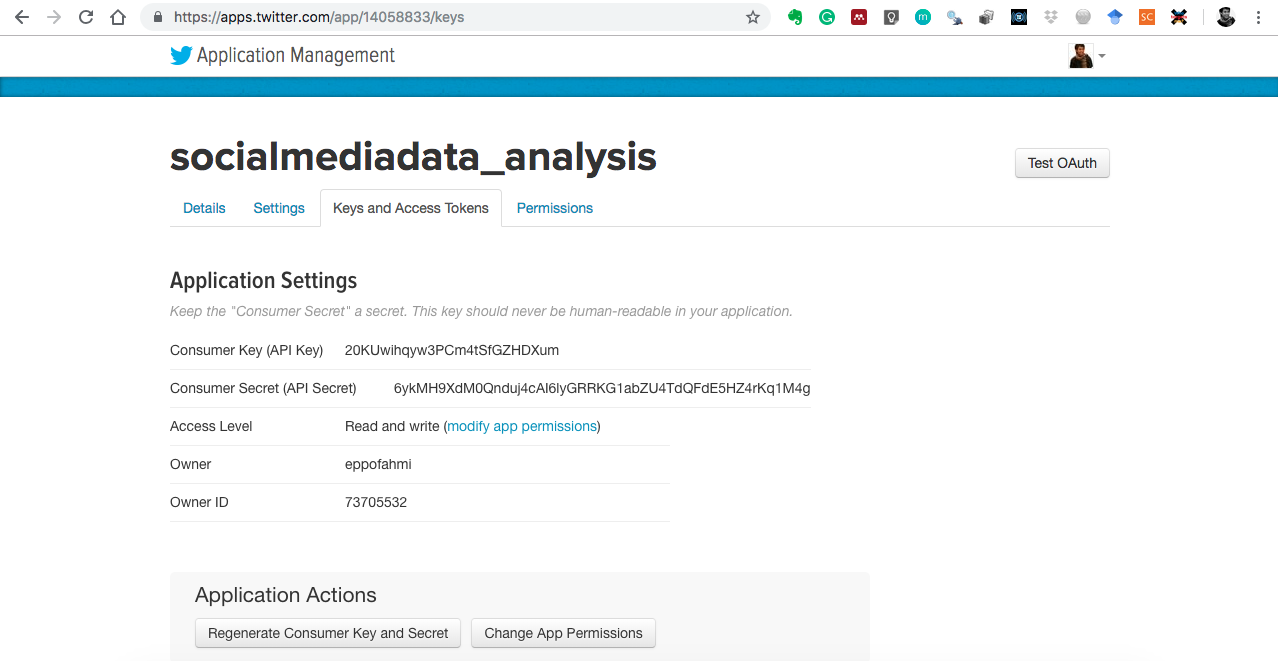
\includegraphics[width=1\linewidth]{images/apiTwitter} \caption{Keys and Access Token Twitter.}\label{fig:intro1}
\end{figure}

Selanjutnya, anda bisa menggunakan script dibawah ini untuk mengatur
penggunaan API dalam R dengan menggunakan library \texttt{twitteR}.
Untuk itu langkah-langkah yang diperlukan adalah:

\begin{enumerate}
\def\labelenumi{\arabic{enumi}.}
\tightlist
\item
  Memanggil library
\end{enumerate}

\begin{Shaded}
\begin{Highlighting}[]
\KeywordTok{library}\NormalTok{(twitteR)}
\end{Highlighting}
\end{Shaded}

\begin{enumerate}
\def\labelenumi{\arabic{enumi}.}
\setcounter{enumi}{1}
\tightlist
\item
  Setting API
\end{enumerate}

\begin{Shaded}
\begin{Highlighting}[]
\NormalTok{api_key <-}\StringTok{ "20KUwihqyw3PCm4tSfGZHDXum"}
\NormalTok{api_secret <-}\StringTok{ "6ykMH9XdM0Qnduj4cAI6lyGRRKG1abZU4TdQFdE5HZ4rKq1M4g"}
\NormalTok{token <-}\StringTok{ "73705532-WlCKXW7Cjd2U2fcSUflTOnoLE0Nrk26gy6xddFzeM"}
\NormalTok{token_secret <-}\StringTok{ "JrUQjxTSx3QSTAGQnL1lnsO2ua8g4LKDV6xzZ4iJW3Rwh"}
\end{Highlighting}
\end{Shaded}

\begin{enumerate}
\def\labelenumi{\arabic{enumi}.}
\setcounter{enumi}{2}
\tightlist
\item
  Setting permission access
\end{enumerate}

\begin{Shaded}
\begin{Highlighting}[]
\KeywordTok{setup_twitter_oauth}\NormalTok{(api_key, api_secret, token, token_secret)}
\end{Highlighting}
\end{Shaded}

Ketika anda menjalankan script di atas pada bagian \texttt{console} akan
ada perintah untuk mengonfirmasi.
\texttt{Tekan\ 1\ dan\ enter\ untuk\ menlanjutkan}.

\begin{enumerate}
\def\labelenumi{\arabic{enumi}.}
\setcounter{enumi}{3}
\tightlist
\item
  Proses ambil data
\end{enumerate}

Dalam proses ini kita membutuhkan akses internet yang akan menentukan
lama atau cepatnya pengambilan data. Di dalam librar \texttt{twitteR}
terdapat beberapa fungsi yang bisa digunakan untuk mengumpulkan data
seperti untuk mendapatkan teks/twit yang berasal dari letak geografis
dan jam tertentu atau untuk mendapatkan timeline sebuah nama akun
(username). Pada kesempatan ini kita akan menggunakan fungsi
\texttt{searchTwitter} untuk mendapatkan twit sebanyak 1000
(\texttt{n\ =\ 1000}) dengan kata kunci tagar \textbf{\#bubarkanbanser}.

\begin{Shaded}
\begin{Highlighting}[]
\NormalTok{banser <-}\StringTok{ }\KeywordTok{searchTwitter}\NormalTok{(}\StringTok{"#bubarkanbanser"}\NormalTok{, }\DataTypeTok{n =} \DecValTok{1000}\NormalTok{) }\CommentTok{# collect tweets}
\NormalTok{banser <-}\StringTok{ }\KeywordTok{twListToDF}\NormalTok{(banser) }\CommentTok{# mengubah format data menjadi data frame}
\KeywordTok{write.csv}\NormalTok{(banser, }\StringTok{"contoh_data.csv"}\NormalTok{) }\CommentTok{# menyimpan data}
\end{Highlighting}
\end{Shaded}

Data yang didapat berupa list, untuk itu pada script bari kedua kita
akan mengubahnya menjaid data frame agar lebih mudah dieksplorasi.
Selanjutnya data yang didapat kita simpan dalam directory yang sudah
kita tentukan sebelumnya saat membuat \texttt{project}.

\hypertarget{eksplorasi-data}{%
\section{Eksplorasi data}\label{eksplorasi-data}}

Di dalam proses mengeksporasi data, hal pertama yang harus diketahui
adalah datanya itu sendiri. Misalnya berapa jumlah observasi, variabel,
jenis variabel dan lain sebagainya. Pada konteks data yang kita dapatkan
dengan metode di atas, terdapat 1000 observasi dan 16 variabel, seperti
dapat dilihat pada bagian \texttt{Environment} (sebelah kanan atas).
Untuk mendapatkan tilikan dengan cepat kita bisa menggunakan fungsi
\texttt{summary} seperti berikut.

\begin{Shaded}
\begin{Highlighting}[]
\KeywordTok{summary}\NormalTok{(banser)}
\end{Highlighting}
\end{Shaded}

Fungsi di atas akan memberikan rangkuman semua variabel atau kolom yang
ada. Di mana dengan melihat rangkuman tersebut di antarnya kita akan
segera mengetahui kapan twit pertama dan terakhir di kirim dalam data.
Selain itu, kita juga bisa mengetahui jenis data pada masing-masing
kolom serta beberapa statistik dasar. Sehingga berdasarkan rangkuman
tersebut kita bisa memutuskan untuk dapat menentukan hal apa yang akan
di eksplorasi terlebih dahulu.

Dengan menggunakan materi sebelumnya (lihat Chapter \ref{explorasi1}),
kita selanjutnya dapat mengeksplorasi akun paling banyak disebut, tagar
paling sering digunakan dan kata paling banyak ditulis kolom text. Di
mana dalam kolom tersebut selain teks twit juga terdapat nama akun yang
disebut oleh pengirimnya, tagar, dan konten lainnya.

\hypertarget{contoh-hasil-kerja}{%
\chapter{Contoh hasil kerja}\label{contoh-hasil-kerja}}

Berikut ini adalah beberapa hasil penelitian yang memanfaatkan data dari
media sosial di berbagai negara dalam berbagai kasus.

\begin{table}

\caption{\label{tab:tableJurnal}Contoh jurnal yang memanfaatkan data dari media sosial}
\centering
\begin{tabular}[t]{l|l|l}
\hline
Judul & Data yang digunakan & DOI\\
\hline
Mapping the Public Agenda with Topic Modeling: The Case of the Russian LiveJournal & 100000 blog post & 10.1002/1944-2866.POI331\\
\hline
Topic Modelling and Event Identification from Twitter Textual Data & 128207 tweet & http://arxiv.org/abs/1608.02519\\
\hline
Politicians and the Policy Agenda: Does Use of Twitter by the U.S. Congress Direct New York Times Content? & 275816 tweet & 10.1002/poi3.120\\
\hline
Soft Data and Public Policy: Can Social Media Offer Alternatives to Official Statistics in Urban Policymaking? & Geotaget tweets from 2 to 19 of June 2014 & 10.1002/poi3.127\\
\hline
Increasing the reach of government social media: A case study in modeling government-citizen interaction on Facebook & 12 Months facebook pages text & 10.1002/poi3.81\\
\hline
Citizen-government collaboration on social media: The case of Twitter in the 2011 riots in England & 296099 tweets & 10.1016/j.giq.2013.10.014\\
\hline
Three dimensions of the public sphere on Facebook & Data on all the active users of Facebook Pages devoted to Polish political parties and politicians & 10.1080/1369118X.2017.1281329\\
\hline
The “Social Side” of Public Policy: Monitoring Online Public Opinion and Its Mobilization During the Policy Cycle & All tweet with \#labuonascuola hashtag & 10.1002/poi3.117\\
\hline
Freedom to hate: social media, algorithmic enclaves, and the rise of tribal nationalism in Indonesia & 37 Pilkada-related public groups on Facebook and tweet with \#Pilkada & 10.1080/14672715.2017.1341188\\
\hline
\end{tabular}
\end{table}

Jika dilihat dari sumber data yang digunakan dalam penelitian-penelitian
di atas (\ref{tab:tableJurnal}), maka kita bisa mengetahui bahwa data
yang digunakan cukup banyak jika dikerjakan secara manual. Selain itu,
beberapa penelitian memang tidak menyebutkan jumlahnya secara spesifik,
tapi umumnya mereka menggunakan data secara menyeluruh atau dengan
sampel yang memadai. Oleh karena itu, mereka banyak memanfaatkan bahwa
pemrogaraman dan bahkan membuat aplikasi khusus untuk mengumpulkan data
seperti dengan judul ``Mapping the Public Agenda with Topic Modeling:
The Case of the Russian LiveJournal'' \citep{KOL}.

\hypertarget{sumber-belajar-mandiri}{%
\chapter{Sumber Belajar Mandiri}\label{sumber-belajar-mandiri}}

\hypertarget{komunitas}{%
\section{Komunitas}\label{komunitas}}

\textbf{1. Kaggle}

Kaggle dapat menjadi salah satu sumber utama bagi siapa saja yang ingin
belajar atau menjadi data scientist.
\href{https://www.kaggle.com/}{Kaggle} menyediakan berbagai jenis data
untuk latihan. Selain itu, \href{https://www.kaggle.com/}{Kaggle} kita
juga bisa belajar dari script yang dibuat oleh orang lain dalam
mengelola data dan mengekstrak informasi dari sebuah data.

\textbf{2. Stackoverflow}

\href{https://stackoverflow.com/}{Stackoverflow} adalah sebuah tempat
bagi orang yang baru belajar hingga sudah mahir untuk bertanya dan
menjawab pertanyaan terkait dengan script dari berbagai bahasa
pemerograman yang ada di dunia. Di sini kita bisa mencari jawab atau
langsung bertanya tentang kendala yang dihadapi dalam menulis script
untuk mendapatkan suatu hasil yang dituju.

\textbf{3. Github}

Walaupun \href{https://github.com/}{GitHub} sebenarnya memiliki fungsi
lain yang dapat dimanfaatkan dalam proses scripting. Namun di sini saya
ingin menekankan bahwa GitHub banyak digunakan oleh para develovers
untuk meletakan scriptnya. Terdapat dua versi, yaitu versi private dan
publik. Untuk versi publik kita bisa menggunakannnya sebagai sumber
belajar dengan mengopi foldernya atau satu persatu.

\hypertarget{free-course}{%
\section{Free Course}\label{free-course}}

Saat ini diinternet banyak kursus dan tutorial daring yang dapat
digunakan sebagai salah satu tempat untuk belajar. Misalnya kita bisa
mencari di youtube, atau juga mengikuti kursus gratis di
\href{https://www.datacamp.com/}{datacamp} atau di
\href{https://www.udemy.com/courses/search/?src=ukw\&q=R}{Udemi}.

\bibliography{book.bib,packages.bib}


\end{document}
